\section{Wnioski}
Tworzenie rozbudowanego oprogramowania do obsługi robota 3D pracującego w~magazynie wysokiego składowania wymaga rozwiązania wielu problemów programistycznych. Autor w pierwszej kolejności zapoznał się z~kursami programowania w~środowisku Step~7 oraz WinCC flexible \cite{kurs1,kurs2,kurs3} dostępnymi w~sieci.

W wyniku realizacji projektu inżynierskiego, którego dotyczy niniejsza praca powstało oprogramowanie dla sterownika przemysłowego Siemens S7-300 sterujące modelem robota firmy Fischertechnik oraz wizualizacja stanu robota wraz ze stanem obsługiwanego magazynu wysokiego składowania.

W pierwszej kolejności powstał kod sterowania pojedynczym silnikiem, który po gruntownym testowaniu podlegał dalszemu rozwojowi. Wszystkie silniki mają możliwość pracowania w trybach: automatycznym, ręcznym z dołączonego do sterownika zadajnika sygnałów dyskretnych oraz ręcznym z poziomu stworzonej wizualizacji. Tak przygotowane oprogramowanie zostało wykorzystane do stworzenia kodu umożliwiającego obsługę zbudowanego przez autora modelu magazynu z wykorzystaniem kolejki zadań do realizacji. Wszystkie operacje wykonywane na magazynie są realizowane z wykorzystaniem zaimplementowanej kolejki FIFO, od momentu kliknięcia przycisku w wizualizacji aż do jej opróżnienia.

Podczas realizacji zostały rozwiązane problemy, z których najtrudniejszym do wyeliminowania zdaniem autora była bezwładność silników. W jej wyniku silnik po wyłączeniu dalej poruszał się przez nieokreślony czas aż do samoistnego zatrzymania. Wyeliminowanie negatywnych efektów tego zjawiska pozwoliło stworzyć w pełni funkcjonalne oprogramowanie spełniające wszelkie wymagania użytkownika.

W~procesie tworzenia oprogramowania autor zapoznał się z~wieloma zagadnieniami typowymi dla sterowników firmy Siemens. Przykładowo, bloki wywoływane podczas startu sterownika (OB100 / OB101 / OB102), z~czego na sterowniku S7-300 dostępnym w~laboratorium dostępny jest tylko blok OB100, czyli tzw. gorący restart (ang. \emph{warm restart}). Wywoływany jest on przy każdym przejściu ze~stanu STOP do RUN/RUN-P oraz podczas uruchamiania po zaniku zasilania.
Kolejne charakterystyczne bloki to~te~wywoływane jako cykliczne przerwania (OB30~do~OB38). Tutaj niestety również występuje ograniczenie i~dostępny jest jedynie blok OB35, wywoływany domyślnie co 100~ms. Częstotliwość wywołania można jednak łatwo zmienić w~konfiguracji sprzętowej jednostki centralnej.

Wykonanie pojedynczego cyklu sterownika stworzonego przez autora oprogramowania w czasie testowania wynosiło od 1 do 3~ms. Czas ten jest zadowalający biorąc pod uwagę, że sterownik bez funkcji użytkownika oraz z~pustym blokiem OB1 ma czas wykonania cyklu równy 1~ms oraz to, że oprogramowanie przynajmniej zdaniem autora jest rozbudowane.
%\begin{figure}[!htb] \centering 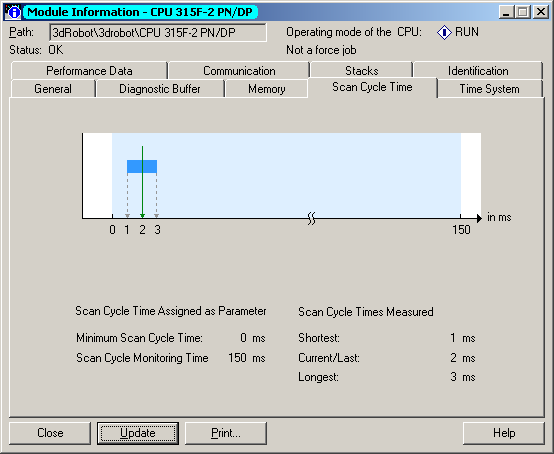
\includegraphics[width=0.6\textwidth]{obrazki/time.PNG} \caption{Czas pojedynczego cyklu sterownika} \end{figure}

Wizualizacja stanu robota stanowi bardzo atrakcyjną formę korzystania z~urządzenia, która jest jednocześnie wyjątkowo przystępna dla osób nie znających zagadnień związanych z programowaniem sterowników przemysłowych. Wizualizacja będzie pełniła ważną rolę w~prezentacji projektu na~potrzeby koła naukowego Industrum.

Bardzo ciekawymi zagadnieniami poznanymi przez autora w czasie realizacji projektu były kwestie bezpieczeństwa. Ważne jest, aby komercyjne i praktyczne projekty realizować ze szczególnym naciskiem na bezpieczną pracę robotów i innych obiektów przemysłowych ze względu na pracujących w ich otoczeniu ludzi oraz na bardzo wysokie koszty zakupu i naprawy takich urządzeń. Przykładowym rozwiązaniem z tego zakresu jest zastosowanie przycisków monostabilnych do załączania silników, co pozwala na natychmiastowy i automatyczny powrót do położenia neutralnego z chwilą ich zwolnienia przez operatora (funkcja „dead-man-control“). Innym rozwiązaniem podnoszącym bezpieczeństwo jest zastosowanie kilku przycisków do awaryjnego zatrzymania pracy modelu. Eliminuje to konieczność precyzyjnego działania w sytuacji kryzysowej.

Autor planuje kontynuować pracę nad projektem na potrzeby koła naukowego Industrum oraz ewentualnie jako projekt magisterski. Ciekawym rozwinięciem byłoby rozbudowanie modelu o~gąsienice albo koła umożliwiając mu tym samym poruszanie. Umożliwiłoby to zastąpienie półkolistego magazynu typowym szeregowym magazynem wysokiego składowania. Magazyn taki mógłby być zdecydowanie większy, a umożliwiając całemu modelowi poruszanie się, również w osi pionowej, zwiększyłoby te możliwości jeszcze bardziej. Dodanie tego elementu wymaga zastosowania technologii bezprzewodowej do komunikacji między modelem, a~sterownikiem. Dobrym pomysłem zdaniem autora byłoby rozbudowanie magazynu o~czujniki oraz platformy wejściowe i~wyjściowe magazynu np. taśmociągi. Biorąc pod uwagę inne modele dostępne w laboratorium bardzo interesująca wydaje się perspektywa połączenia ich wszystkich w~jedną całość, uzyskując w~ten sposób dość rozbudowaną linię produkcyjną.
